\section{Java enterprise edition}

Java enterprise edition is a platform aimed at the development, release and maintenance of three-tier web applications.
\begin{figure}[H]
    \centering
    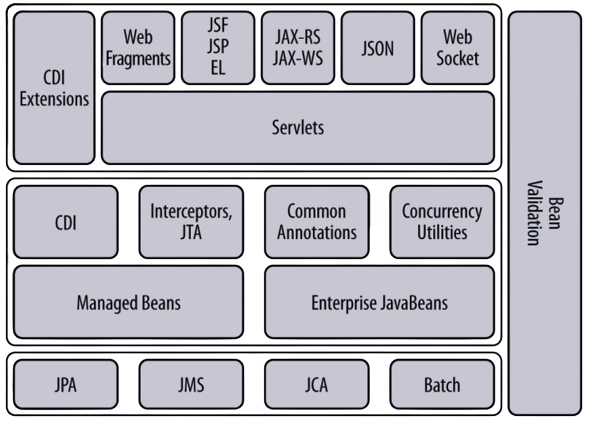
\includegraphics[width=0.5\linewidth]{images/jee.png}
    \caption{Jakarta EE stack}
\end{figure}
The main elements of this platform are: 
\begin{itemize}
    \item JDBC: this API was the first industry standard for database independent connectivity between Java and the database. Thanks to this API we can:
        establish a connection with a database, send SQL statements, and process the results. 
    \item Servlet, that are the Java technology for the presentation tier in web application. The servlets: 
        offer a component-based, platform independent method for building web-based applications, have access to other Java APIs to access enterprise databasesa 
        and are executed within a container for concurrency control and lifecycle management. 
    \item Jakarta Enterprise Beans: it is the technology used in the server. They enable the development of distributed, transactional, secure and portable applications. 
        EJB components can be used by the web front-end to interact with the business functions and data access services. 
    \item Java Persistence API: it is the specification of an interface for mapping relational data to object oriented data in Java. 
        It comprises: the API implementation package javax.persistence, the Java compatible query language Java Persistence Query Language, and the specification of the metadata for defining object
        relational mappings. 
    \item Java Transaction API: it is an API for managing transactions in Java. It allows a component to start, commit and rollback transactions in a resource agnostic way. 
        With this technology, Java components can manage multiple resources in a single transaction with a unique interaction model.
\end{itemize}
\begin{example}
    To extract data from a database using JPA we use: 
    \begin{lstlisting}[style=Java]
public List<Mission> findMissionsByUser(int userId) {
Reporter reporter = em.find(Reporter.class, userId);
List<Mission> missions = reporter.getMissions();
return missions;
}
    \end{lstlisting}
    To insert data in a database using JPA we use: 
    \begin{lstlisting}[style=Java]
public void createMission(Date startDate, int days, String destination, String description, int reporterId) {
Reporter reporter = em.find(Reporter.class, reporterId);
Mission mission = new Mission(startDate, days, destination, description, reporter);
reporter.addMission(mission);
em.persist(reporter);
}        
    \end{lstlisting}
    To modify data in a database using JPA we use: 
    \begin{lstlisting}[style=Java]
public void reportMission(int missionId, MissionStatus missionStatus) {
Mission mission = em.find(Mission.class, missionId);
mission.setStatus(MissionStatus.REPORTED);
}
    \end{lstlisting}
\end{example}